\section{Investigation of a Single Inverter Module}
\label{chap:curr_driven_rect}

\subsection{Effect on Power Device Stress}

In physical realization of power electronics circuit, the parasitic inductances of the layout is an important consideration especially for the paths carrying switched current. In Fig. \ref{fig:SingleModuleInductanceMap}, an inductance map is given for the designed three phase inverter system as shown in Fig.\ref{fig:invertermodule}. In an inverter structure, two loops are critical for device and capacitance stresses. As shown in Fig. \ref{fig:SingleModuleInductanceMap}, the power loop includes two switches and the phase capacitor. When the phase current transfers from one of the switch to other switch in a half-bridge, the power loop parasitic inductances cause either a voltage overshoot or undershoot on a switch's drain-source terminals as much voltage as $L_p*di/dt$. Considering the high current rise and fall time capability of GaN HEMTs, i.e. high di/dt, the power loop inductance is very the most important factor for device stress.

%%Neden GaN kullanıyoruz, GaN olunca burda nasıl bir zorluk oluştu?

%%Teorisinden bahsedelim => Ldi/dt

%%Power loop sadece etken

%%Experimental resultlar (Vds overshoot) => A ve B fazı karşılaştırılabilir

%%Sıkıntılı durumda neler yapılabilir? (hangi parametreler etken)

%% Experimental result figür ve yorumlanması


\subsection{Effect on DC link Capacitor Stress}

As seen in Fig. \ref{fig:invertermodule}, a distributed DC bus architecture is designed on each module where each half-bridge leg has its own capacitor in close proximity. These capacitors are used to supply and sink the current ripple during switching periods. The power loop inductances are not effective on these capacitors' stress assuming ceramic capacitors with small ESL are placed in much closer proximity.

When an ideal inverter is considered with a single DC bus capacitor, it is seen that commutation of all the phases are reflected to this capacitor. When the capacitors are distributed and the parasitic inductances are of considerable amount, the stress of individual capacitors increase on the peak of corresponding phase current due to the longer path which the other capacitors have. This situation is visualised in Fig. \ref{fig:single_module_curr_ripple}. This results in higher capacitor RMS currents than analytically calculated and must be taken into account as the selected capacitor temperature may increase too much, eventually shortening its lifetime. On the other hand, this effect is not significantly reflected to the voltage ripple.

%% solda a fazı inductance olmayan akım waveformu ve olan hali (at a peak phase)
%% sagda 3 faz yes inductance rms ler ve no inductance case 1 kapasitör rmsi üstüste (1 period) --- bunu ekleyecez fig olarak

\begin{figure}[tb]
\minipage{0.49\textwidth}
  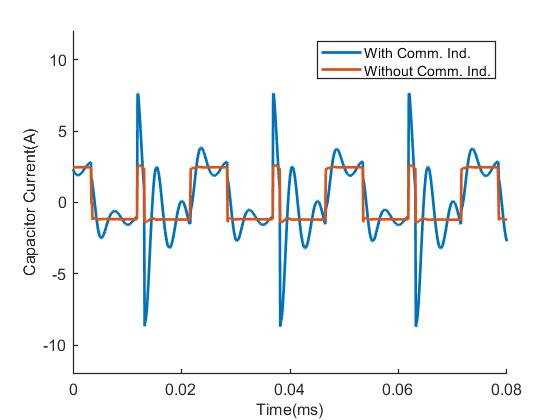
\includegraphics[width=\linewidth]{figures/single_module_curr_ripple.jpg}
  \caption{DC bus capacitor current ripple with and without commutation loop inductances}\label{fig:single_module_curr_ripple}
\endminipage\hfill
\minipage{0.49\textwidth}
  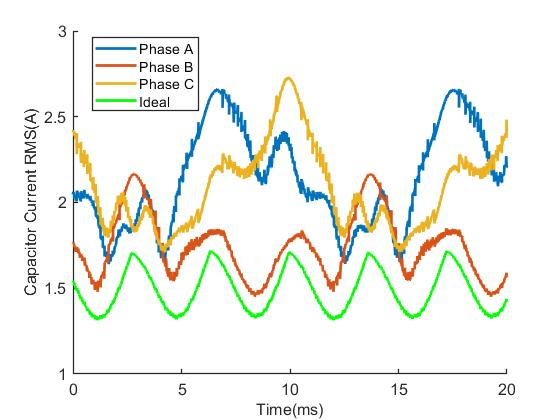
\includegraphics[width=\linewidth]{figures/CapacitorCurrentRMS.jpg}
  \caption{Waveform of RMS values of capacitor currents with and without commutation inductances}\label{fig:CapacitorCurrentRMS}
\endminipage
\end{figure}

Stress sharing olayı ve arada doğan farkın önemi

Mümkünse voltage ripple experimental datası

